%% COSC 520 Assignment 3 - Vertex cover and greedy graph coloring
%% ACM Small format with the ACM, journal and copyright information removed.
%% Compile with pdfLaTeX + BibTeX (Overleaf default).

\documentclass[acmsmall,nonacm]{acmart}

\setcopyright{none}
\settopmatter{printacmref=false}
\renewcommand\footnotetextcopyrightpermission[1]{}
\pagestyle{plain}

\usepackage{tikz}

\newcommand{\code}[1]{\texttt{#1}}
\newcommand{\OPT}{\mathrm{OPT}}

\begin{document}

\title{Vertex Cover and Greedy Coloring on Hard Benchmark Graphs: Two Simple Heuristics Each, Measured Against Exact Optima}
\subtitle{COSC 520 Assignment 3 --- Student number 84298512}

\author{Ahmed Elgazwy}
\email{ahmed.elgazwy@ubc.ca}
\affiliation{%
  \institution{University of British Columbia}
  \city{Kelowna}
  \state{British Columbia}
  \country{Canada}}

\begin{abstract}
Vertex cover and graph coloring are NP-hard, and in practice they are attacked with simple heuristics. We implement two for each in Python, from scratch: the basic matching-based vertex cover and Pitt's randomized version, and greedy coloring along the natural vertex order and along the smallest-last order. We prove that all four run in $\Theta(n+m)$ time with $\Theta(n)$ extra space, and measure them on the 36 BHOSLIB/FRB benchmark graphs (up to 7.4 million edges), whose chromatic number and, for their complements, minimum vertex cover are known exactly. The measured growth is linear (log-log slopes 0.94--1.09). The randomized vertex cover costs the same as the basic one and finds smaller covers in every family; on a perfect matching it is optimal while the basic algorithm is exactly twice the optimum. Smallest-last coloring takes 5--6 times as long as natural coloring but uses 1.45--1.73 times the chromatic number, against 2.9--5.6 times for the natural order on randomly relabeled graphs. We also find that the vertex numbering of the FRB files hands the natural order the planted solution: in the published numbering it uses exactly the chromatic number on all 36 graphs.
\end{abstract}

\keywords{vertex cover, approximation algorithms, randomized algorithms, graph coloring, greedy coloring, smallest-last ordering, degeneracy, BHOSLIB}

\maketitle

%% ---------------------------------------------------------------------------
\section{Introduction}

A \emph{vertex cover} of a graph $G=(V,E)$ is a set of vertices that touches
every edge, and a \emph{proper coloring} gives adjacent vertices different
colors. Finding a smallest vertex cover and the fewest colors, the chromatic
number $\chi(G)$, are both NP-hard~\cite{karp1972}. Neither problem can be
approximated well: vertex cover cannot be approximated within a factor of 1.36
unless P${}={}$NP~\cite{dinur2005}, nor within $2-\varepsilon$ under the Unique
Games Conjecture~\cite{khot2008}, and the chromatic number cannot be
approximated within $n^{1-\varepsilon}$~\cite{zuckerman2007}. In practice both
problems are therefore attacked with simple, fast heuristics.

This report studies two such heuristics for each problem, implemented by hand
in Python: the basic matching-based vertex cover algorithm and its randomized
version~\cite{pitt1985}, and greedy coloring along the natural vertex order and
along the \emph{smallest-last} order~\cite{matula1983}. It makes four
contributions:
\begin{itemize}
  \item linear-time implementations of the four algorithms, with 121 unit tests that compare them against literal versions of the lecture pseudo-code and against brute-force optima;
  \item a time and space analysis of each algorithm, in particular of the smallest-last ordering (Section~\ref{sec:complexity});
  \item a benchmark on all 36 BHOSLIB/FRB graphs~\cite{xu2007,rossi2015}, used in two forms whose exact optima are known, so that every result is measured against the true optimum rather than a bound (Sections~\ref{sec:setup}--\ref{sec:results});
  \item the observation that the vertex numbering of the FRB files leaks the planted solution to the ``arbitrary'' natural order, and a correction by random relabeling (Section~\ref{sec:numbering}).
\end{itemize}

\noindent\textbf{Code:} \url{https://github.com/ahmedelgazwy/Advanced_DS_assignment_3}\\
\textbf{Dataset:} \url{https://networkrepository.com/bhoslib.php} (BHOSLIB, Network Repository)

%% ---------------------------------------------------------------------------
\section{The Algorithms}
\label{sec:algorithms}

Throughout, $n=|V|$, $m=|E|$, $\Delta$ is the largest degree, and $\OPT$ is the
size of a minimum vertex cover.

\subsection{Basic vertex cover}

The lecture algorithm~\cite{cormen2009,skiena2020,salavatipour2013} repeatedly selects an arbitrary remaining edge $(u,v)$,
adds \emph{both} $u$ and $v$ to the cover $C$, and deletes every edge incident
to $u$ or $v$. Our implementation scans the edge list once, in input order,
and adds both endpoints of each edge that has neither endpoint in $C$ yet. The
two are equivalent: an edge is deleted by the lecture loop exactly when one of
its endpoints enters $C$, so the next uncovered edge of the scan is the next
edge the loop would select. A unit test checks that both produce the same cover
on 150 random graphs.

\textbf{Approximation ratio 2.} The selected edges form a matching $M$, since
both endpoints of a selected edge were outside $C$. The matching is maximal,
because every edge ends up with an endpoint in $C$. Any vertex cover must
contain a distinct endpoint of each edge of $M$, so $\OPT\ge|M|$ and
$|C|=2|M|\le 2\,\OPT$. The bound is tight: on $k$ disjoint edges, or on
$K_{k,k}$, the algorithm takes all $2k$ vertices while $\OPT=k$.

\subsection{Randomized vertex cover}

Pitt's algorithm~\cite{pitt1985} scans the same edges in the same order, but
adds \emph{one} endpoint of each uncovered edge, chosen by a fair coin. Keeping
the edge order identical makes the coin the only difference between the two
algorithms. Both algorithms have weighted versions~\cite{pitt1985,baryehuda1981},
which this report does not study.

\textbf{Expected ratio 2.} Fix an optimal cover $C^*$. Each selected edge has
an endpoint in $C^*$, so the coin picks a vertex of $C^*$ with probability at
least $\frac12$. Let $G_t$ ($B_t$) indicate that edge $t$ is selected and the
picked vertex is (is not) in $C^*$. Given the history, $E[B_t]\le E[G_t]$, and
$\sum_t G_t\le|C^*|$ because a picked vertex covers all its edges and is never
picked again. By linearity of expectation, $E|C|=\sum_t E[G_t+B_t]\le
2\,|C^*|$. The guarantee holds only in expectation: on a star whose edges list
the leaf first, a single run can pick several leaves before the center. On a
perfect matching, however, the randomized algorithm is always optimal.

\subsection{Greedy coloring}

Greedy coloring visits the vertices in some order and gives each vertex the
smallest color (0, 1, 2, \ldots) not used by its already-colored neighbors.
Following Gebremedhin et al.~\cite{gebremedhin2009}, define the \emph{back
degree} of a vertex in an order $\pi$ as its number of neighbors placed before
it, and $B_\pi$ as the largest back degree. A vertex sees at most its back
degree in blocked colors, so greedy coloring uses at most $B_\pi+1\le\Delta+1$
colors. The basic algorithm uses the \emph{natural order} $0,1,\ldots,n-1$ of
the input. It can be very poor: on the crown graph ($K_{k,k}$ minus a perfect
matching) numbered $a_0,b_0,a_1,b_1,\ldots$ it uses $k$ colors for a bipartite
graph, and on a binomial tree with $n$ vertices numbered in post-order it uses
$\log_2 n+1$ colors for a tree~\cite{gyarfas1988}.

\subsection{The smallest-last ordering}
\label{sec:sl}

The csc09 paper~\cite{gebremedhin2009} describes four degree-based orderings:
largest first~\cite{welsh1967}, incidence degree, dynamic largest first and
smallest last; the graph coloring page of Chiarandini~\cite{chiarandini} lists
further heuristics such as DSATUR~\cite{brelaz1979}. We chose \emph{smallest last} (SL)~\cite{matula1983}. It builds
the order from the end: the last vertex $v_n$ is a vertex of minimum degree in
$G$; it is removed, $v_{n-1}$ is a vertex of minimum degree in what remains,
and so on. The back degree of each vertex in the final order is its degree when
it was removed. Figure~\ref{fig:sl-example} shows the process on a small graph.

%% ---- Written by Ahmed Elgazwy: begin ----
We selected the smallest-last ordering because, among the four orderings discussed in the CSC09 paper, it is the only one with a clear optimization objective: minimizing the maximum back degree across all possible vertex orderings. This gives greedy coloring a guarantee of using at most \(d+1\) colors, where \(d\) is the graph's degeneracy. This is never worse than the \(\Delta+1\) bound obtained with an arbitrary ordering and can be significantly better in practice. For example, it guarantees a 2-coloring for trees and uses at most 6 colors for planar graphs. Another advantage is that the ordering can be computed in linear time using a bucket queue, allowing both coloring algorithms in our comparison to run in \(\Theta(n+m)\) time, with the only difference being the vertex ordering. We chose it over DSATUR, which can often produce colorings with fewer colors, because DSATUR selects vertices dynamically rather than following a fixed ordering and requires \(\Theta((n+m)\log n)\) time when implemented with a heap. Finally, smallest-last is independent of the input vertex numbering, making it particularly interesting for evaluating adversarial examples. We also found this property to be relevant when working with the FRB instances.
%% ---- Written by Ahmed Elgazwy: end ----

\textbf{The degeneracy guarantee.} The \emph{degeneracy} $d$ of $G$ is the
largest $k$ such that $G$ has a subgraph of minimum degree $k$. Every order has
$B_\pi\ge d$: in such a subgraph $H$, the last vertex of $H$ in $\pi$ has at
least $d$ neighbors before it. SL achieves $B_\pi=d$, because each vertex is
removed with the minimum degree of the remaining subgraph, which is at most
$d$. So SL minimizes $B_\pi$ over all $n!$ orders~\cite{gebremedhin2009}, and
greedy coloring along it uses at most $d+1$ colors. The bound $d+1$ can be far
below $\Delta+1$: a star has $\Delta=n-1$ but $d=1$, and planar graphs have
$d\le5$.

\begin{figure}[t]
\centering
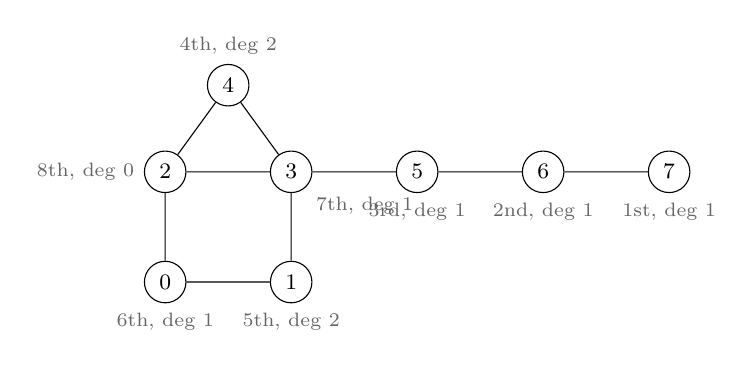
\begin{tikzpicture}[v/.style={circle,draw,inner sep=1pt,minimum size=15pt,font=\footnotesize},
                    r/.style={font=\scriptsize,text=black!60}]
  \node[v,label={[r]below:6th, deg 1}] (0) at (0,0) {0};
  \node[v,label={[r]below:5th, deg 2}] (1) at (1.6,0) {1};
  \node[v,label={[r]left:8th, deg 0}] (2) at (0,1.4) {2};
  \node[v,label={[r]below right:7th, deg 1}] (3) at (1.6,1.4) {3};
  \node[v,label={[r]above:4th, deg 2}] (4) at (0.8,2.5) {4};
  \node[v,label={[r]below:3rd, deg 1}] (5) at (3.2,1.4) {5};
  \node[v,label={[r]below:2nd, deg 1}] (6) at (4.8,1.4) {6};
  \node[v,label={[r]below:1st, deg 1}] (7) at (6.4,1.4) {7};
  \draw (0)--(1) (0)--(2) (1)--(3) (2)--(3) (2)--(4) (3)--(4) (3)--(5) (5)--(6) (6)--(7);
\end{tikzpicture}
\caption{Smallest-last on a small graph. Each vertex is labeled with the step at which it was removed and its degree at that moment. The coloring order is the reverse of the removal order, $2,3,0,1,4,5,6,7$, and the largest degree at removal gives the degeneracy $d=2$, so greedy coloring uses at most 3 colors (the triangle 2--3--4 needs exactly 3).}
\label{fig:sl-example}
\end{figure}

%% ---------------------------------------------------------------------------
\section{Complexity Analysis}
\label{sec:complexity}

We use the word-RAM model. The graph is stored once as an edge list in input
order ($2m$ integers) and once in compressed sparse row (CSR) form: an array
of $n+1$ offsets and an array of $2m$ neighbor ids. Building both takes
$\Theta(n+m)$ time and space. This is the input; the space figures below count
the \emph{extra} space each algorithm allocates. Table~\ref{tab:complexity}
summarizes the results.

\textbf{Vertex cover, both versions.} One pass over the $m$ edges with $O(1)$
work per edge: two lookups in a membership array, and for a selected edge at
most two writes, two appends and, for the randomized version, one random bit.
The membership array costs $\Theta(n)$ to allocate. Time $\Theta(n+m)$; extra
space $\Theta(n)$ (the membership flags and the cover itself, at most $n$
vertices).

\textbf{Greedy coloring, any order.} A \code{forbidden} array of $n+1$ entries
is reused for every vertex with a \emph{stamp}: \code{forbidden[c] = v} means
that color $c$ is taken by a neighbor of $v$, so the array never needs
clearing. Coloring $v$ reads its $\deg(v)$ neighbors and then scans the colors
$0,1,\ldots$ until one is free; the scan stops after at most $\deg(v)+1$ steps,
since at most $\deg(v)$ colors are blocked. In total
$\sum_v(\deg(v)+1)=2m+n$, so the time is $\Theta(n+m)$ and the extra space
$\Theta(n)$ (the colors and the stamps).

\textbf{The smallest-last ordering.} A naive implementation searches for a
minimum-degree vertex at every step, which costs $\Theta(n^2)$. A bucket queue
reduces this to $\Theta(n+m)$~\cite{matula1983,batagelj2003}. Our layout keeps
four arrays: \code{deg[v]} (current degree), \code{vert} (the vertices not yet
removed, sorted by current degree), \code{pos[v]} (the position of $v$ in
\code{vert}) and \code{start[k]} (the first position of degree $k$).
\begin{enumerate}
  \item \emph{Bin sort} the vertices by degree into \code{vert}, \code{pos} and \code{start}: $\Theta(n+\Delta)=\Theta(n)$, since $\Delta<n$.
  \item For $i=0,\ldots,n-1$: remove $v=\code{vert}[i]$, a vertex of minimum current degree because \code{vert} is sorted from position $i$ on.
  \item For each neighbor $u$ of $v$ not yet removed, with current degree $k$: swap $u$ with the first vertex of bucket $k$, advance \code{start[k]} by one (so $u$ becomes the last vertex of bucket $k-1$), and decrement \code{deg[u]}. The array stays sorted.
  \item The coloring order is the removal order reversed; the degeneracy $d$ is the largest degree seen at a removal.
\end{enumerate}
Each vertex is removed once and each of the $2m$ adjacency entries is examined
once, when its vertex is removed, with $O(1)$ work: a comparison, at most one
swap and two counter updates. One subtlety is that a bucket's stored start can
fall behind the removed prefix when degrees drop below the current minimum; it
is then clamped to $i+1$ when read, which is $O(1)$. A unit test checks the
defining property (every removal has minimum remaining degree) on 100 random
graphs. \textbf{Time} $\Theta(n+m)$. \textbf{Extra space} $\Theta(n)$: the
arrays \code{deg}, \code{pos} and \code{vert} of $n$ entries each, and
\code{start} of $\Delta+2\le n+1$ entries, about $4n$ words in total. Greedy
coloring along the SL order then adds another $\Theta(n+m)$ pass, so SL
coloring costs a constant factor more than natural coloring, with the same
growth.

\begin{table}[t]
\caption{Time and extra space (beyond the $\Theta(n+m)$ graph) of the four algorithms, and their quality guarantees.}
\label{tab:complexity}
\small
\begin{tabular}{@{}llll@{}}
\toprule
Algorithm & Time & Extra space & Guarantee \\
\midrule
Basic vertex cover & $\Theta(n+m)$ & $\Theta(n)$ & $|C|=2|M|\le2\,\OPT$ (tight) \\
Randomized vertex cover & $\Theta(n+m)$ & $\Theta(n)$ & $E|C|\le2\,\OPT$ \\
Greedy, natural order & $\Theta(n+m)$ & $\Theta(n)$ & at most $\Delta+1$ colors \\
Smallest-last order alone & $\Theta(n+m)$ & $\Theta(n)$, about $4n$ words & $B_\pi=d$, the minimum over all orders \\
Greedy, smallest-last order & $\Theta(n+m)$ & $\Theta(n)$ & at most $d+1\le\Delta+1$ colors \\
\bottomrule
\end{tabular}
\end{table}

%% ---------------------------------------------------------------------------
\section{Experimental Setup}
\label{sec:setup}

\textbf{Dataset.} We use the 36 FRB graphs of the BHOSLIB benchmark hosted by
Network Repository~\cite{rossi2015}: seven families of five instances
(\code{frb30-15} to \code{frb59-26}) and \code{frb100-40}
(Table~\ref{tab:dataset}). Instance \code{frbN-K} was generated by
Model~RB~\cite{xu2000,xu2007}. It consists of $N$ groups of $K$ vertices, with
a planted solution, and the vertices of group $g$ are numbered $gK,\ldots,gK+K-1$.
Network Repository publishes the dense \emph{clique form} (\code{clq}); its
complement, the \emph{independent-set form} (\code{mis}), is the form the
original benchmark uses for vertex cover. We use both, because each has an
exactly known optimum:
\begin{itemize}
  \item \code{clq}: no edge joins two vertices of the same group (we checked all 36 files), so the groups form a proper $N$-coloring; the planted solution is an $N$-clique, so at least $N$ colors are needed. Hence $\chi=N$.
  \item \code{mis}: every group is a clique, so an independent set has at most one vertex per group; the planted solution has $N$. Hence the maximum independent set has $N$ vertices and $\OPT=NK-N$.
\end{itemize}
The two forms also span a wide range of sizes, from $1.8\times10^4$ to
$7.4\times10^6$ edges. Since $\OPT$ is $1-1/K$ of all vertices (93--97.5\%),
\emph{any} cover of a \code{mis} graph is within a factor $K/(K-1)\le1.072$
of optimal; the vertex cover comparison on FRB is therefore made within this
narrow band.

\begin{table}[t]
\caption{The FRB graphs (edge counts are ranges over the five instances of a family) and their exact optima.}
\label{tab:dataset}
\small
\begin{tabular}{@{}lrrrrrr@{}}
\toprule
Family & $N$ & $K$ & $n$ & $m$, \code{clq} & $m$, \code{mis} & $\chi$ (\code{clq}) / $\OPT$ (\code{mis}) \\
\midrule
frb30-15 & 30 & 15 & 450 & 83,151--83,231 & 17,794--17,874 & 30 / 420 \\
frb35-17 & 35 & 17 & 595 & 148,572--148,873 & 27,842--28,143 & 35 / 560 \\
frb40-19 & 40 & 19 & 760 & 246,801--247,325 & 41,095--41,619 & 40 / 720 \\
frb45-21 & 45 & 21 & 945 & 386,854--387,795 & 58,245--59,186 & 45 / 900 \\
frb50-23 & 50 & 23 & 1,150 & 579,607--580,640 & 80,035--81,068 & 50 / 1,100 \\
frb53-24 & 53 & 24 & 1,272 & 714,048--714,229 & 94,127--94,308 & 53 / 1,219 \\
frb59-26 & 59 & 26 & 1,534 & 1,048,800--1,049,829 & 125,982--127,011 & 59 / 1,475 \\
frb100-40 & 100 & 40 & 4,000 & 7,425,226 & 572,774 & 100 / 3,900 \\
\bottomrule
\end{tabular}
\end{table}

\textbf{The vertex numbering leaks the solution.}
\label{sec:numbering}
Because each group of the \code{clq} form is an independent set numbered
consecutively, greedy coloring in the file's natural order colors the graph
group by group and recovers the planted $N$-coloring. The natural order of the
file is therefore not ``arbitrary''. The same holds for the edge order that the
vertex cover algorithms scan. We therefore measure quality both in the file's
numbering and on randomly relabeled copies: a random permutation of the vertex
ids and of the edge order (five copies per graph, three for \code{frb100-40}).

\textbf{Synthetic graphs.} The FRB graphs have at most 4,000 vertices. To
measure growth over three orders of magnitude we also use uniform random graphs
$G(n,5n)$ (average degree 10) for $n=10^3,\ldots,10^6$ in 1--2--5 steps.

\textbf{Measurement.}
All runs used one machine: an Intel Core i7-11800H (2.3\,GHz, 8 cores) with 16\,GiB of RAM, Windows~11 and CPython 3.10.2; the full benchmark takes about 15 minutes.
Each time is the median of five runs (three for graphs with more than
$2\times10^6$ edges) with the garbage collector paused; loading and building
the graph are not timed. The randomized vertex cover is run with 30 seeds per
graph. Extra memory is the peak allocation measured by \code{tracemalloc} in
separate runs. The whole benchmark is reproduced by
\code{python -m scripts.run\_benchmarks}.

%% ---------------------------------------------------------------------------
\section{Results}
\label{sec:results}

Table~\ref{tab:results} summarizes the measurements per FRB family;
Table~\ref{tab:hypotheses} checks the predictions of the analysis.

\begin{table}[t]
\caption{Measured performance per FRB family (mean over its instances). Times are for the published \code{clq} form. Quality is on randomly relabeled copies and relative to the exact optimum: cover size$/\OPT$ on the \code{mis} form, colors$/\chi$ on the \code{clq} form.}
\label{tab:results}
\footnotesize
\setlength{\tabcolsep}{4pt}
\begin{tabular}{@{}lr|rrrr|rr|rr@{}}
\toprule
 & & \multicolumn{4}{c|}{Time, \code{clq} form (ms)} & \multicolumn{2}{c|}{Cover$/\OPT$} & \multicolumn{2}{c}{Colors$/\chi$} \\
Family & $m$ (\code{clq}) & basic & random. & natural & SL & basic & random. & natural & SL \\
\midrule
frb30-15 & 83,198 & 7.5 & 7.7 & 10.7 & 60.5 & 1.058 & 1.048 & 2.93 & 1.67 \\
frb35-17 & 148,791 & 13.0 & 12.7 & 18.0 & 104 & 1.052 & 1.041 & 3.25 & 1.72 \\
frb40-19 & 247,041 & 20.3 & 20.5 & 31.1 & 166 & 1.046 & 1.037 & 3.45 & 1.70 \\
frb45-21 & 387,403 & 31.5 & 31.9 & 43.8 & 260 & 1.042 & 1.034 & 3.73 & 1.71 \\
frb50-23 & 580,218 & 50.4 & 49.8 & 68.5 & 431 & 1.038 & 1.031 & 3.91 & 1.68 \\
frb53-24 & 714,121 & 59.5 & 57.5 & 89.0 & 476 & 1.037 & 1.030 & 4.02 & 1.54 \\
frb59-26 & 1,049,452 & 87.9 & 92.1 & 124 & 698 & 1.034 & 1.027 & 4.20 & 1.64 \\
frb100-40 & 7,425,226 & 463 & 464 & 902 & 5,420 & 1.022 & 1.018 & 5.60 & 1.45 \\
\bottomrule
\end{tabular}
\end{table}

\subsection{Running time}

Figure~\ref{fig:frb-runtime} plots the running time of the four algorithms on
all 72 FRB graphs. All four grow linearly in $n+m$: the fitted log-log slopes
are 1.09 (basic), 1.06 (randomized), 0.94 (natural) and 1.01 (smallest-last). On \code{frb100-40}, with 7.4 million edges, the two vertex
cover algorithms take 0.46\,s each, natural coloring 0.90\,s and
smallest-last coloring 5.4\,s. The two vertex cover algorithms cost the
same: the extra random bit of the randomized version is offset by the fewer
vertices it adds.

Smallest-last coloring costs 5.3--6.3 times as much as natural coloring on the
\code{clq} graphs (3.9--5.3 times on the sparser \code{mis} graphs). Its greedy
pass costs the same as the natural one, about 125\,ns per element of $n+m$, but
computing the order costs about 560\,ns per element: for each adjacency entry it
reads the neighbor's position, degree and bucket start, and may swap two
entries, while the greedy pass reads one color.

Figure~\ref{fig:scaling} shows the cost per element of $n+m$ on random graphs
$G(n,5n)$, where the analysis predicts flat lines. The vertex cover algorithms
stay at 64--92\,ns from $n=10^3$ to $10^6$ (slopes 1.01; 0.49\,s and 0.54\,s at
$n=10^6$). The coloring algorithms are flat up to about $10^5$ vertices and then
rise gently (slopes 1.06 and 1.07; smallest-last takes 8.2\,s at $n=10^6$),
once their per-vertex arrays outgrow the CPU caches and each adjacency entry
reads a random vertex's entry from main memory. This is a memory-hierarchy
effect outside the RAM model; the operation count is linear.

\begin{figure}[t]
  \centering
  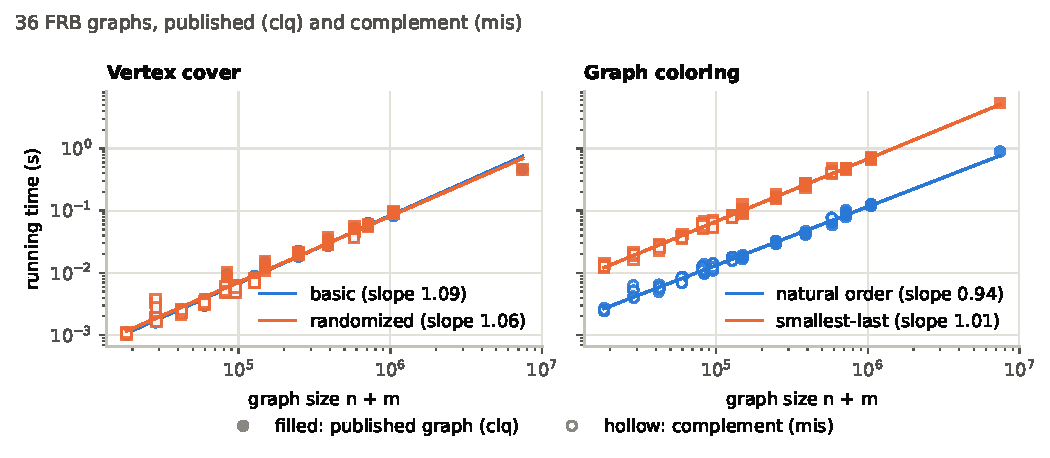
\includegraphics[width=\linewidth]{figures/frb_runtime.pdf}
  \caption{Running time on the 36 FRB graphs in both forms (log-log), with the fitted power law of each algorithm. A slope of 1 means linear time.}
  \label{fig:frb-runtime}
\end{figure}

\begin{figure}[t]
  \centering
  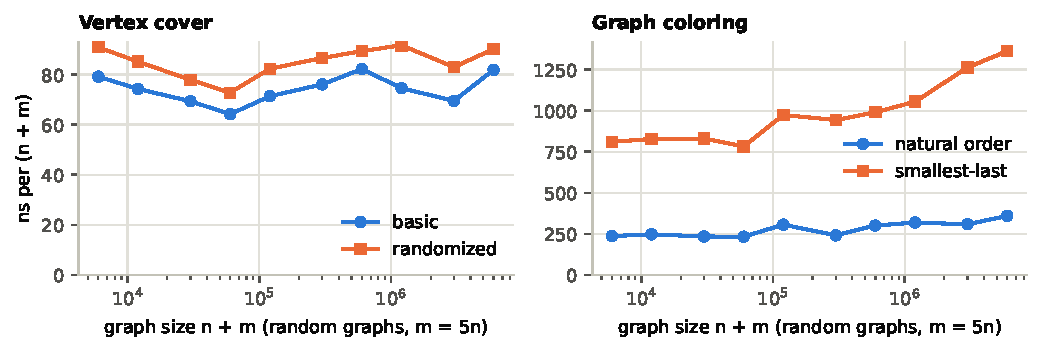
\includegraphics[width=\linewidth]{figures/scaling_per_element.pdf}
  \caption{Cost per element of $n+m$ on random graphs $G(n,5n)$. Linear-time algorithms give flat lines.}
  \label{fig:scaling}
\end{figure}

\subsection{Vertex cover quality}

Figure~\ref{fig:vc-quality} compares the cover sizes with the exact optimum on
the \code{mis} graphs. All ratios lie between 1.018 and 1.071, below the
ceiling $n/\OPT$, so a more telling measure is the \emph{excess} $|C|-\OPT$ as
a share of the largest possible excess, $n-\OPT=N$. In the file's edge order
the basic algorithm is at the ceiling: it takes \emph{every} vertex of
\code{frb53-24}, \code{frb59-26} and \code{frb100-40}. On relabeled copies its
excess falls to 82--86\%. The randomized algorithm is better in every family
and both numberings; on relabeled copies its excess is 66--72\% (for example
440.3 vertices against 444.5 on \code{frb30-15}, $\OPT=420$), with a standard
deviation below one vertex over 30 seeds.

The worst-case families show the full gap the analysis allows. On a perfect
matching of 1,000 edges the basic algorithm takes exactly $2\,\OPT$ and the
randomized one the optimum, for every seed; on $K_{100,100}$ they take 200 and
185 on average (165--198), against $\OPT=100$. On a star with 1,000 leaves
listed leaf first both take 2 on average, but the randomized algorithm took 8
in its worst run: its bound holds only in expectation.

\begin{figure}[t]
  \centering
  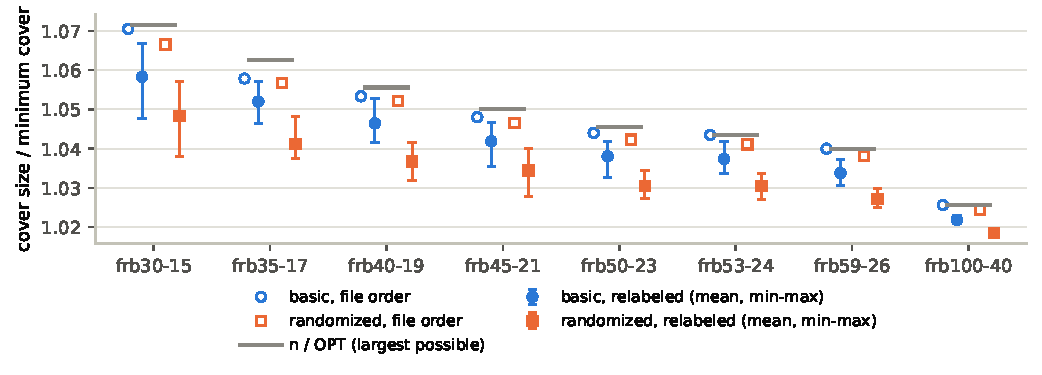
\includegraphics[width=\linewidth]{figures/vc_quality.pdf}
  \caption{Vertex cover of the \code{mis} graphs relative to the exact optimum. Hollow: the file's edge order; filled: relabeled copies (mean, with the range). The gray bars mark the largest possible ratio, $n/\OPT$.}
  \label{fig:vc-quality}
\end{figure}

\subsection{Coloring quality}

Figure~\ref{fig:coloring-quality} compares the color counts with the exact
chromatic number of the \code{clq} graphs. In the file's numbering, natural
greedy coloring uses exactly $\chi=N$ colors on all 36 graphs: as explained in
Section~\ref{sec:setup}, the numbering hands it the planted coloring. On
relabeled copies, where the order is truly arbitrary, it uses 2.9 times $\chi$
on \code{frb30-15} (87.8 colors for $\chi=30$), rising to 5.6 times on
\code{frb100-40} (560 for $\chi=100$). Smallest-last ignores the numbering: it
uses 1.45--1.73 times $\chi$ in both numberings (50.2 colors on \code{frb30-15},
145.3 on \code{frb100-40}), 1.7 to 3.9 times fewer than the natural order on
the same relabeled graphs, an advantage that generally grows with the graph.

The degeneracy bound guarantees little on these dense graphs ($d+1$ is 338 on
\code{frb30-15}, close to $\Delta+1$), and smallest-last does far better than
it. On sparse graphs the guarantee is decisive: on the binomial tree $B_{12}$
(4,096 vertices) the natural order uses 13 colors and smallest-last 2, and on
the 200-vertex crown graph 100 colors against 2, the optimum.

\begin{figure}[t]
  \centering
  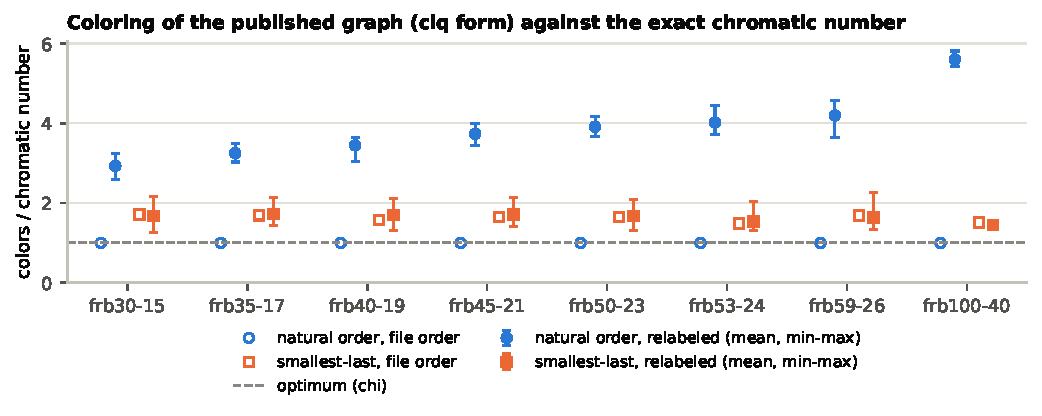
\includegraphics[width=\linewidth]{figures/coloring_quality.pdf}
  \caption{Colors used on the \code{clq} graphs relative to the exact chromatic number. Hollow: the file's numbering; filled: relabeled copies (mean, with the range). The dashed line is the optimum.}
  \label{fig:coloring-quality}
\end{figure}

\subsection{Memory}

The extra memory of every algorithm is proportional to $n$ and independent of
$m$, as predicted. On $G(n,5n)$ the peak extra allocation per vertex is the
same at $n=10^4$, $10^5$ and $10^6$: 31\,bytes for the randomized vertex cover,
34 for the basic one, 52 for natural coloring and 48 for the smallest-last
order. These are CPython constants: a list entry is an 8-byte pointer and
integers above 256 are 28-byte objects, while flags and the smallest-last work
arrays take 1 or 4 bytes per entry. On the FRB graphs, with 185 to 684 edges
per vertex, the cost is similar (22--65\,bytes per vertex). The graph itself
takes $8n+16m$ bytes, about 119\,MB for \code{frb100-40}.

\begin{table}[t]
\caption{The hypotheses of the analysis (repository file \code{docs/theory.md}) against the measurements.}
\label{tab:hypotheses}
\footnotesize
\begin{tabular}{@{}p{0.43\linewidth}p{0.53\linewidth}@{}}
\toprule
Hypothesis & Measured \\
\midrule
H1: all four algorithms run in $\Theta(n+m)$; the log-log slope of time against $n+m$ is about 1. & \textbf{Confirmed.} Slopes 0.94--1.09 on FRB and 1.01--1.07 on $G(n,5n)$; the coloring passes cost up to 1.6 times more per element at $10^6$ vertices (cache misses). \\
H2: basic and randomized vertex cover differ in time by a constant factor only. & \textbf{Confirmed.} The same cost on FRB (84\,ns per element each); 0.49\,s against 0.54\,s at $n=10^6$. \\
H3: smallest-last coloring costs a constant 2--3 times natural coloring. & \textbf{Constant, but larger:} 5.3--6.3 times on \code{clq} and 3.9--5.3 on \code{mis}, because the ordering pass costs about 4.5 greedy passes per element. \\
H4: basic vertex cover $\le2\,\OPT$; on FRB \code{mis} within $K/(K-1)$. & \textbf{Confirmed.} Exactly $2\,\OPT$ on the perfect matching and $K_{100,100}$; 1.022--1.071 on FRB. \\
H5: randomized vertex cover finds smaller covers on average. & \textbf{Confirmed} in all 8 families and both numberings; optimal on the perfect matching. \\
H6: smallest-last uses at most $d+1$ colors and fewer than the natural order. & \textbf{Confirmed} on relabeled copies (1.7--3.9 times fewer) and on the adversarial families; \textbf{not} in the file's numbering, where the natural order recovers $\chi$. \\
H7: neither coloring reaches $\chi$ on FRB \code{clq}. & \textbf{Confirmed} for smallest-last (1.45--1.73\,$\chi$); the natural order reaches $\chi$ only through the numbering. \\
H8: extra memory grows with $n$, not with $m$. & \textbf{Confirmed.} A constant 31--52 bytes per vertex from $n=10^4$ to $10^6$; similar on FRB graphs with up to 684 edges per vertex. \\
\bottomrule
\end{tabular}
\end{table}

%% ---------------------------------------------------------------------------
\section{Discussion}
\label{sec:discussion}

\textbf{Benchmark design matters as much as the algorithms.} The most
striking result is not an algorithm's: in the FRB files' numbering the basic
greedy coloring is optimal on all 36 graphs, and 2.9 to 5.6 times worse on the
same graphs renumbered at random. A benchmark that kept the published numbering
would conclude that the natural order is perfect. Generated instances often
number their vertices in construction order, so ``arbitrary'' orders should be
randomized before such comparisons.

\textbf{Which algorithm to use.} For vertex cover the randomized algorithm is
the better default: it costs the same, produced a smaller cover in every FRB
family, and is optimal on matchings, where the basic algorithm is twice the
optimum. The basic algorithm keeps one advantage: its factor-2 bound holds for
every run, while the randomized bound holds only in expectation (the star
example). For coloring, smallest-last is worth its constant factor of about
five to six in time: the order is still computed in linear time, it is immune to the
numbering, it used 1.7--3.9 times fewer colors on the FRB graphs, and it is
optimal on trees and crown graphs. Both remain far from optimal on these hard
instances (45--73\% above $\chi$), which are designed so that no polynomial
heuristic finds the planted solution.

\textbf{Implementation effects.} The first benchmark run measured the basic
vertex cover three times slower than the randomized one at $10^6$ vertices.
The cause was a Python \code{set} for the covered vertices against a
\code{bytearray} in the randomized version; with the same \code{bytearray}
both cost the same, as the final run shows. The storage of the smallest-last
work arrays is a genuine trade-off: lists hold pointers to integer objects,
while flat \code{array}s hold integers inline but create an integer object on
every read. On the dense FRB graphs, which fit in the CPU cache, lists are
faster (423 against 589\,ms on \code{frb59-26-1}); at $10^6$ vertices flat
arrays are (5.8 against 9.0\,s), and only they keep the cost per element flat.
We kept the flat arrays, which inflates the smallest-last ratio on FRB.

\textbf{Threats to validity.} All times come from one machine and CPython, and
a compiled implementation could change the ratio between the ordering and the
greedy pass. The FRB graphs are dense, so vertex cover is compared within the
narrow band below $K/(K-1)$. Graphs with more than $2\times10^6$ edges were
timed three times instead of five.

%% ---------------------------------------------------------------------------
\section{Conclusion}

We implemented two heuristics for vertex cover and two for graph coloring,
proved their linear time and space bounds, and measured them against the exact
optima of the 36 BHOSLIB/FRB graphs. The measurements confirm the analysis:
all four algorithms scale linearly with $n+m$, use space linear in $n$, and
respect their guarantees. Within those guarantees, the randomized vertex cover
found smaller covers than the basic one at the same cost, and the
smallest-last order used 1.7--3.9 times fewer colors than an arbitrary order
for about five to six times the time. Finally, the FRB files' own vertex numbering
reveals the planted coloring, so fair comparisons of order-dependent
heuristics on these benchmarks need randomly relabeled copies.

%% ---------------------------------------------------------------------------
\section*{Use of Generative AI}

This work was produced with the assistance of Claude Code (Anthropic, Claude
Opus 5.5), as allowed by the course policy with disclosure.
\begin{itemize}
  \item \textbf{The author} wrote the bodies of \code{basic\_vertex\_cover} and \code{greedy\_coloring} and the hand-worked unit tests in \code{tests/test\_author\_cases.py} (each marked ``Written by Ahmed Elgazwy'' in the code), and the paragraph explaining the choice of the smallest-last ordering in Section~\ref{sec:sl}. The author also approved the plan, including the smallest-last ordering and the use of both dataset forms, directed the work in phases and reviewed it (recorded in \code{docs/review\_log.md}). One edit inside the author's code was made by the assistant with the author's approval: the \code{set} of covered vertices in \code{basic\_vertex\_cover} became a \code{bytearray} (same logic; marked in the code).
  \item \textbf{The assistant} wrote the remaining code (graph structure, file readers, randomized vertex cover, smallest-last ordering, generators, demo, benchmark and plotting scripts), the other unit tests, and drafted this report.
\end{itemize}

\bibliographystyle{ACM-Reference-Format}
\bibliography{references}

\end{document}
